% Figure : crise S0366 jouée sous les quatre politiques (données : ip_timeseries.csv, lot A)
\begin{tikzpicture}
\begin{axis}[
  width=0.93\textwidth, height=7cm,
  xmin=-10, xmax=45, ymin=0.80, ymax=1.02,
  xlabel={Jours depuis le début de la perturbation}, ylabel={Performance de service $\mathrm{IP}(t)$},
  xtick={-10,0,10,20,30,40}, ytick={0.80,0.85,0.90,0.95,1.00},
  yticklabel style={/pgf/number format/.cd,fixed,fixed zerofill,precision=2,use comma},
  tick label style={font=\scriptsize}, label style={font=\small},
  grid=major, grid style={black!8},
  legend style={font=\scriptsize, draw=none, fill=white, fill opacity=0.9, text opacity=1, at={(0.98,0.04)}, anchor=south east, cells={anchor=west}},
  every axis plot/.append style={line width=1.1pt}]
  \fill[black!5] (axis cs:0,0.80) rectangle (axis cs:21,1.02);
  \node[font=\scriptsize, text=black!60, anchor=north] at (axis cs:10.5,1.018) {fermeture d'Atlanta (21 jours, sévérité 0,95)};
  \addplot[polnone, const plot mark left] table[x=jour,y=none] {figures/data/fig4_S0366.dat};
  \addlegendentry{Sans réaction (IPC 1,47)}
  \addplot[poltard, dotted, const plot mark left] table[x=jour,y=tardif] {figures/data/fig4_S0366.dat};
  \addlegendentry{Tardif (IPC 0,93)}
  \addplot[polprud, dashed, const plot mark left] table[x=jour,y=prudent] {figures/data/fig4_S0366.dat};
  \addlegendentry{Prudent (IPC 0,66)}
  \addplot[polreac, const plot mark left] table[x=jour,y=reactif] {figures/data/fig4_S0366.dat};
  \addlegendentry{Réactif (IPC 0,29)}
  % jours de détection
  \addplot[only marks, mark=triangle*, mark size=3pt, polreac] coordinates {(0,0.8838)};
  \addplot[only marks, mark=triangle*, mark size=3pt, polprud] coordinates {(1,0.8468)};
  \addplot[only marks, mark=triangle*, mark size=3pt, poltard] coordinates {(3,0.8466)};
  \node[font=\scriptsize, anchor=north east, text=black!65] at (axis cs:44.5,0.985) {$\blacktriangle$ : jour de détection de chaque profil};
\end{axis}
\end{tikzpicture}


 % 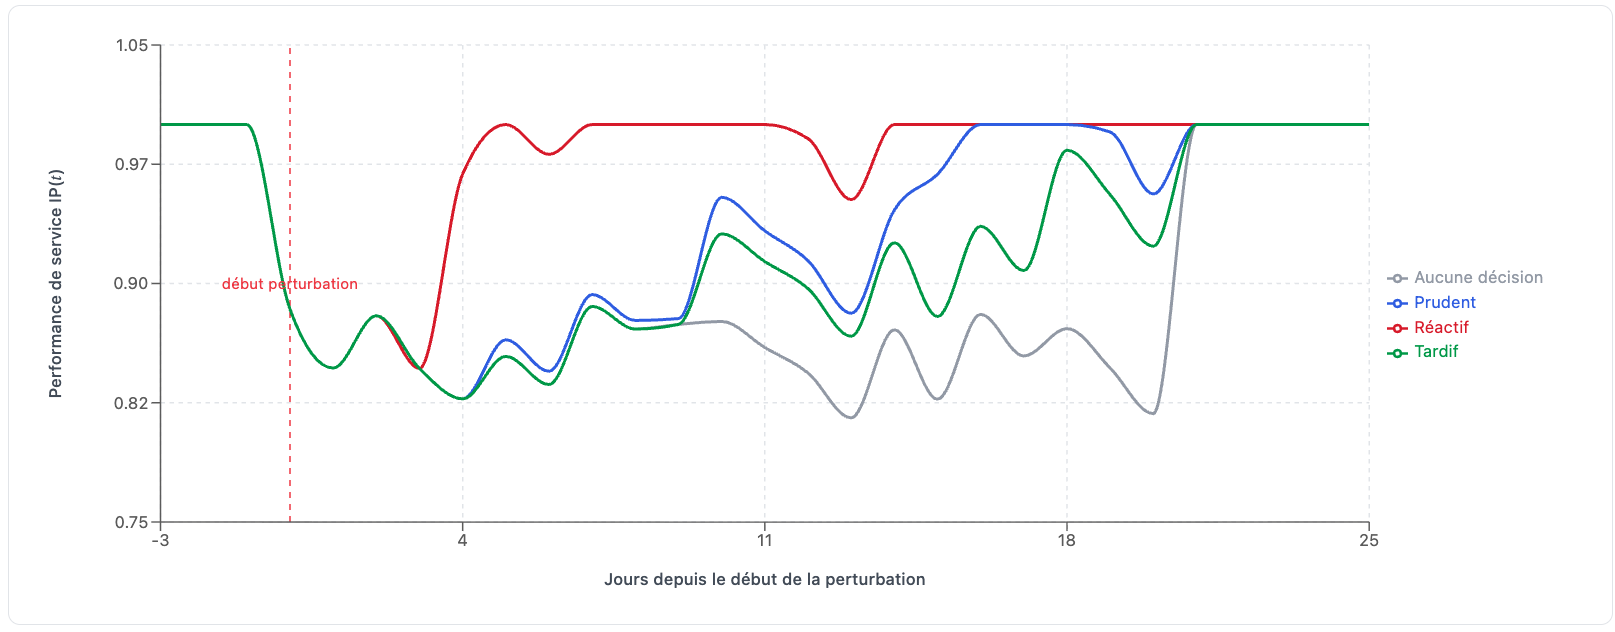
\includegraphics[width=1\textwidth]{fig_crise_S0366.png}

